\section{Incircle family}

A 3-periodic interscribed in a CAP pair with incircle is shown in \cref{fig:06-six-caps}(top middle).

Recall that for this pair, Cayley implies the inradius $r=\frac{{a}{b}}{a+b}$. Also recall that in \cref{prop:03-n3-incircle-R}, we show that incircle 3-periodics have invariant circumradius $R=(a+b)/2$ and that the locus of the circumcenter $X_3$ is a circle of radius $d=(a-b)/2$ centered on $X_1$, see \cref{fig:03-incircle-circum}.

The next 4 propositions are illustrated in \cref{fig:06-incircle-x2456}.

\begin{figure}
    \centering
    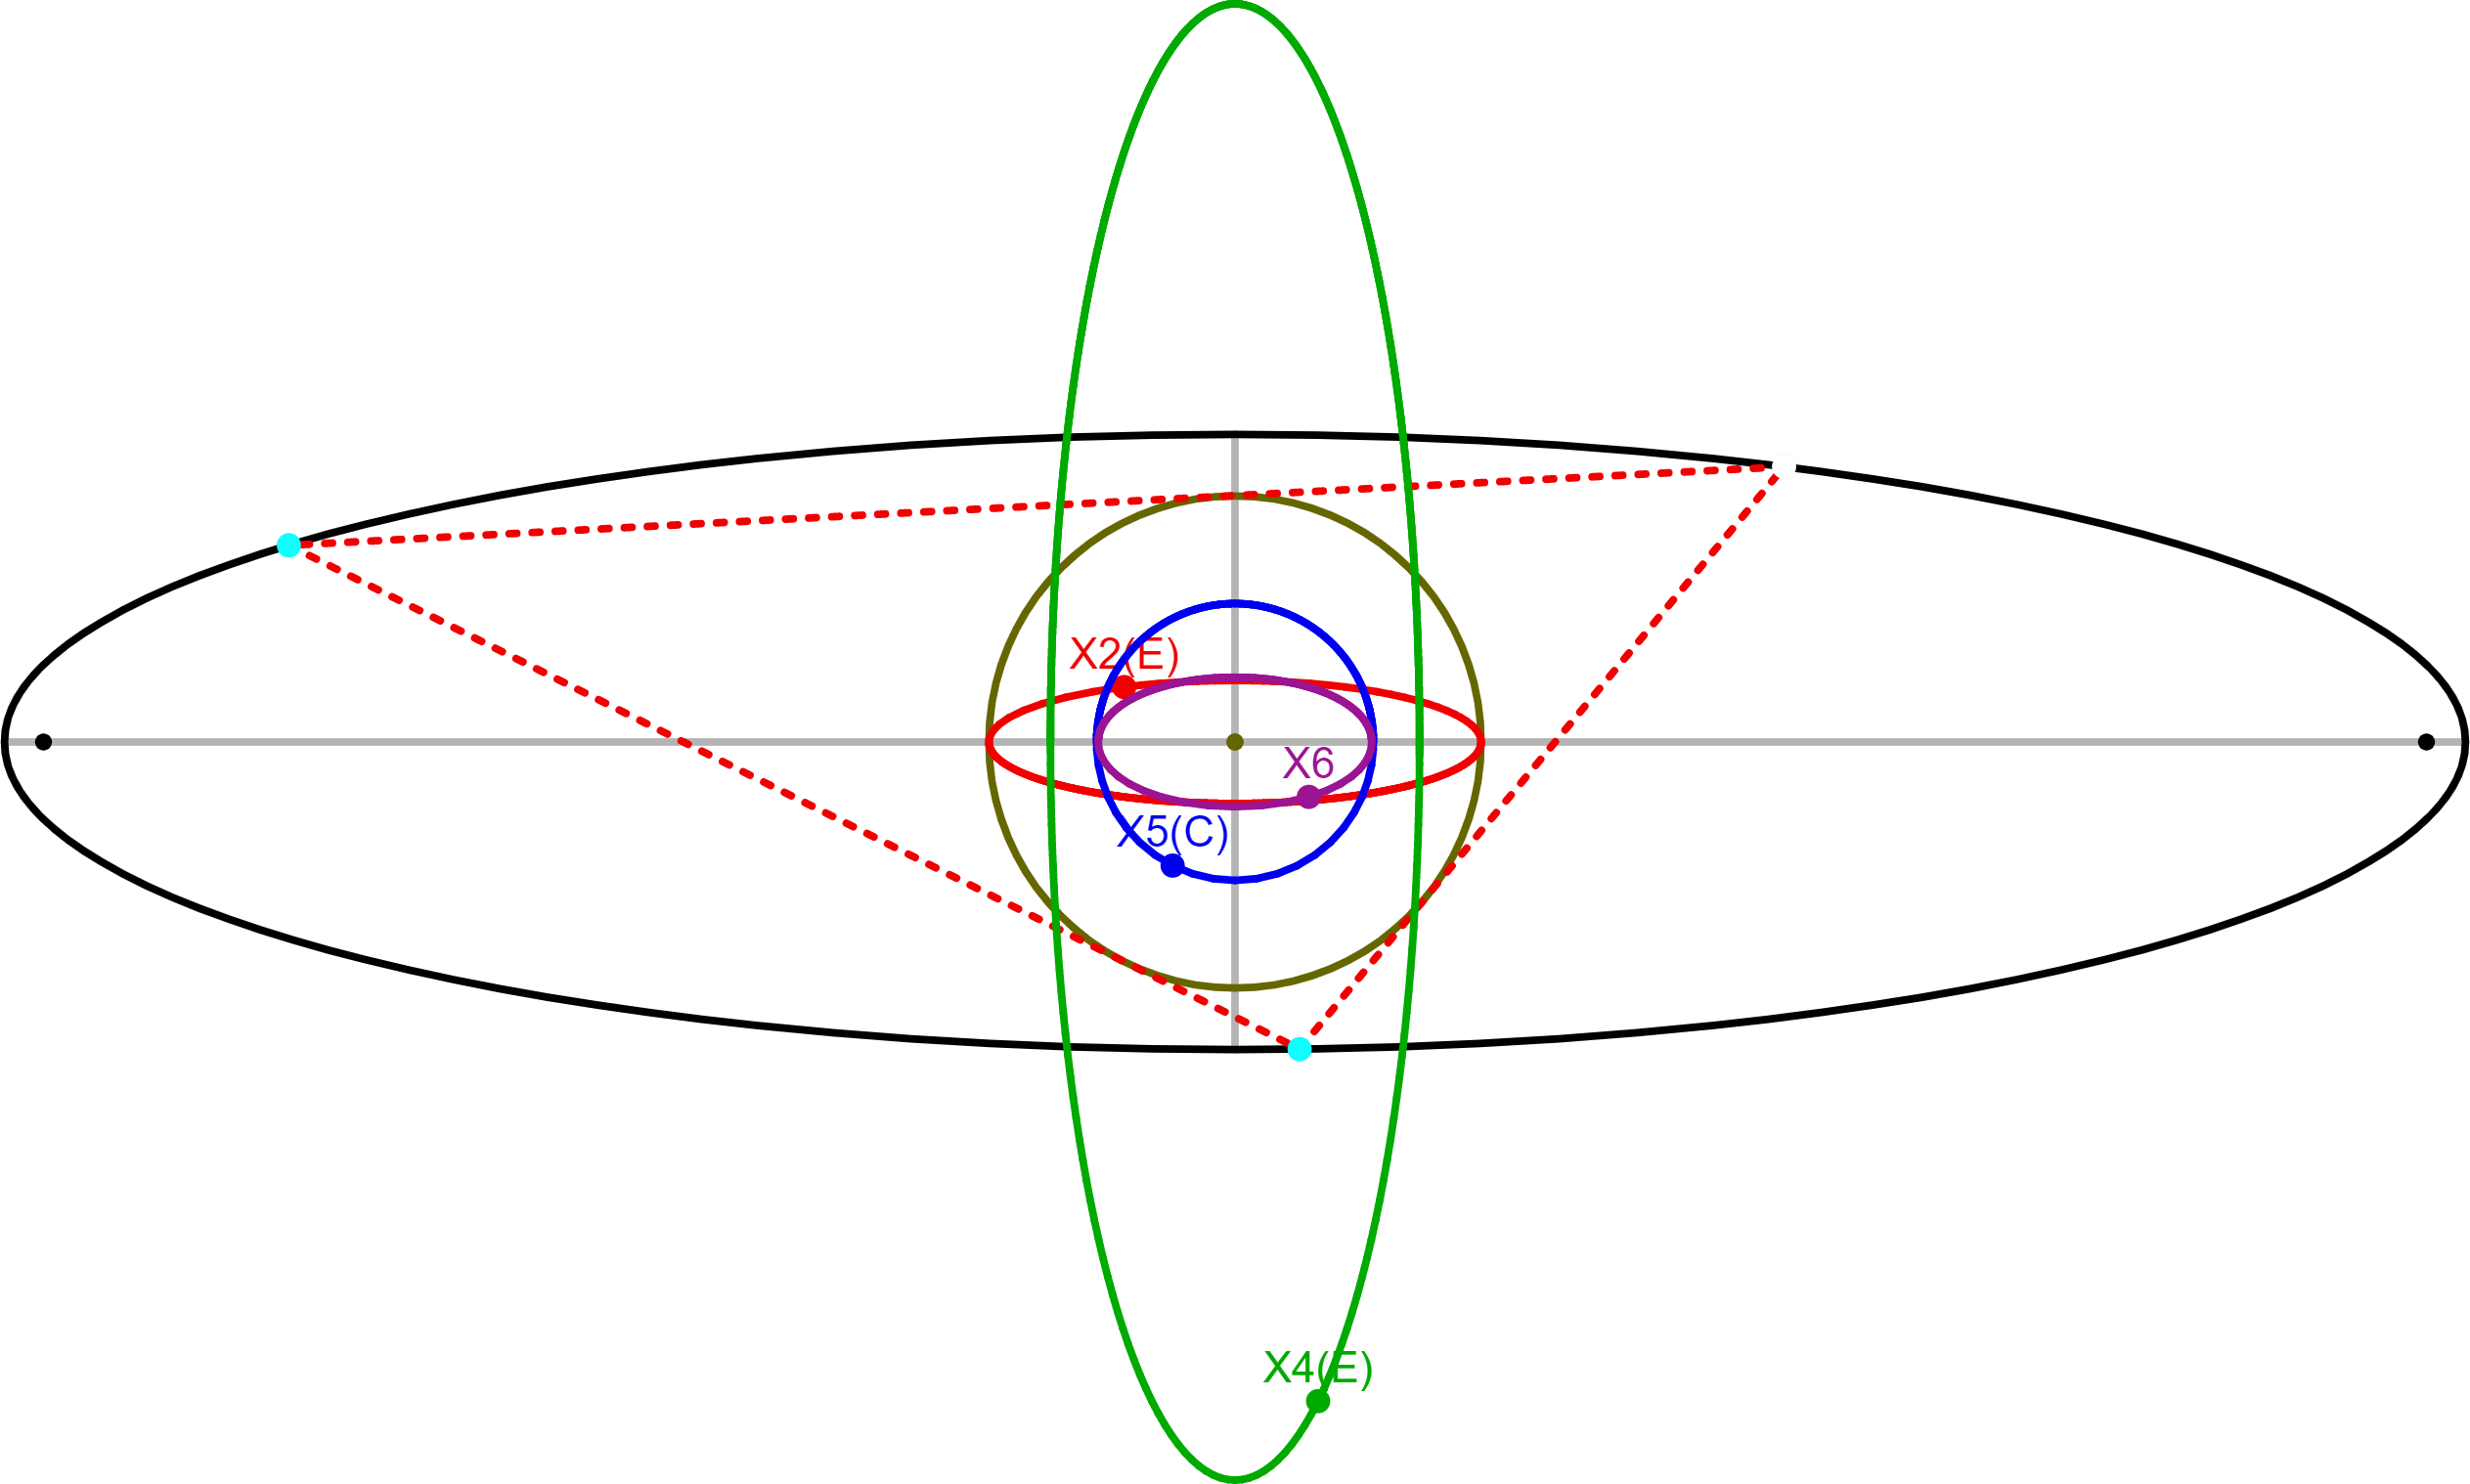
\includegraphics[width=\textwidth]{pics_06_020_incircle_x2456.png}
    \caption{Loci of $X_k$, $k=$2,4,5,6 over incircle 3-periodics. These are ellipses for all but $X_5$ whose locus is a circle. \href{https://bit.ly/2SvuMpi}{Live 1}, \href{https://bit.ly/3fpO098}{Live 2}}
    \label{fig:06-incircle-x2456}
\end{figure}

\begin{proposition}
Over incircle 3-periodics, the locus of the barycenter $X_2$ is an ellipse with axes $a_2=a(a - b)/(3a + 3b)$ and $b_2=b(a - b)/(3a + 3b)$ centered on $O=X_1$.
 \label{prop:06-incircle-X2-locus}
\end{proposition}

\begin{proof}
Follows from \cref{sec:03-cap-vtx-param}.
\end{proof}

\begin{proposition}
Over incircle 3-periodics, the locus of the orthocenter $X_4$ is an ellipse of axes $a_4=(a - b)b/(a + b) $ and $b_4=(a - b)a/(a + b)$
 centered  on $O=X_1$.
\label{prop:06-x4-locus}
\end{proposition}

\begin{proposition}
Over incircle 3-periodics, the locus of the center $X_5$ of the 9-point circle is a circle of radius $d=\frac{(a-b)^2}{4(a+b)}$
  centered on $O=X_1$.
\label{prop:X5}
\end{proposition}

\begin{proof}
Direct, analogous to \cite[Thm.3]{garcia2020-new-properties}.
\end{proof}

\begin{proposition}
Over incircle 3-periodics, the locus of $X_6$ is a quartic given by the following implicit equation:

\begin{align*}
    &   \left( b \left( b+2\,a \right)  \left( {a}^{2}+2\,ab+3\,{b}^{2}
 \right)  {x}^{2}+a \left( a+2\,b \right)  \left( 3\,{a}^{2}+2\,ab+{b}
^{2} \right) {y}^{2} \right) ^{2}\\
&-{a}^{2}{b}^{2} \left( a-b \right) ^{
2} \left( {b}^{2} \left( b+2\,a \right) ^{2}{x}^{2}+{a}^{2} \left( a+2
\,b \right) ^{2}{y}^{2} \right) =0
\end{align*}
\end{proposition}


